% Chapter 1

\chapter{Analysis of the Data Stream} % Main chapter title

\label{ChapterAnalysis} % Change X to a consecutive number; for referencing this chapter elsewhere, use \ref{ChapterX}

%----------------------------------------------------------------------------------------
%	BEGING CHAPTER

%\underline{PERSONNAL REF}
%{\color{red}[see Neutron measurements at IP2I with Ge
%bolometers.pdf]}
%
%\href{https://elog.ipnl.in2p3.fr/manoir/R%26D+Cryo+LIO/51}{https://elog.ipnl.in2p3.fr/manoir/R\%26D+Cryo+LIO/51}
%
%\underline{WEAK REF}
%
%{\color{red}[see NeutronMeasurementCampaign.pdf]}
%
%OFNote.pdf
%
%\underline{STRONG REF}
%
%68Ge-68Ga-Decay.pdf


%----------------------------------------------------------------------------------------



\section{Pre-processing and Data format}
\label{par:data-format}
\label{par:of-processing}

The data were initially saved as streams: the voltage value of the heat channel and the four ionization channel are saved for each time step in the acquisition with a sampling frequency of 400Hz. 

These voltage values are extracted by an analog-to-digital conversion system and thus expressed in \textbf{A}nalog-to-\textbf{D}igital conversion \textbf{U}nit (ADU).
These data streams are then processed by an \textbf{O}ptimal \textbf{F}iltering (OF) software called NEPAL. A filter based on the signal PSD and the noise PSD in the bolometer is applied to the stream. Time windows of 1s centered on a triggering events are selected with an amplitude threshold on the filtered stream (see Figure \ref{fig:raw-of-signal}).

\begin{figure}
\centering
%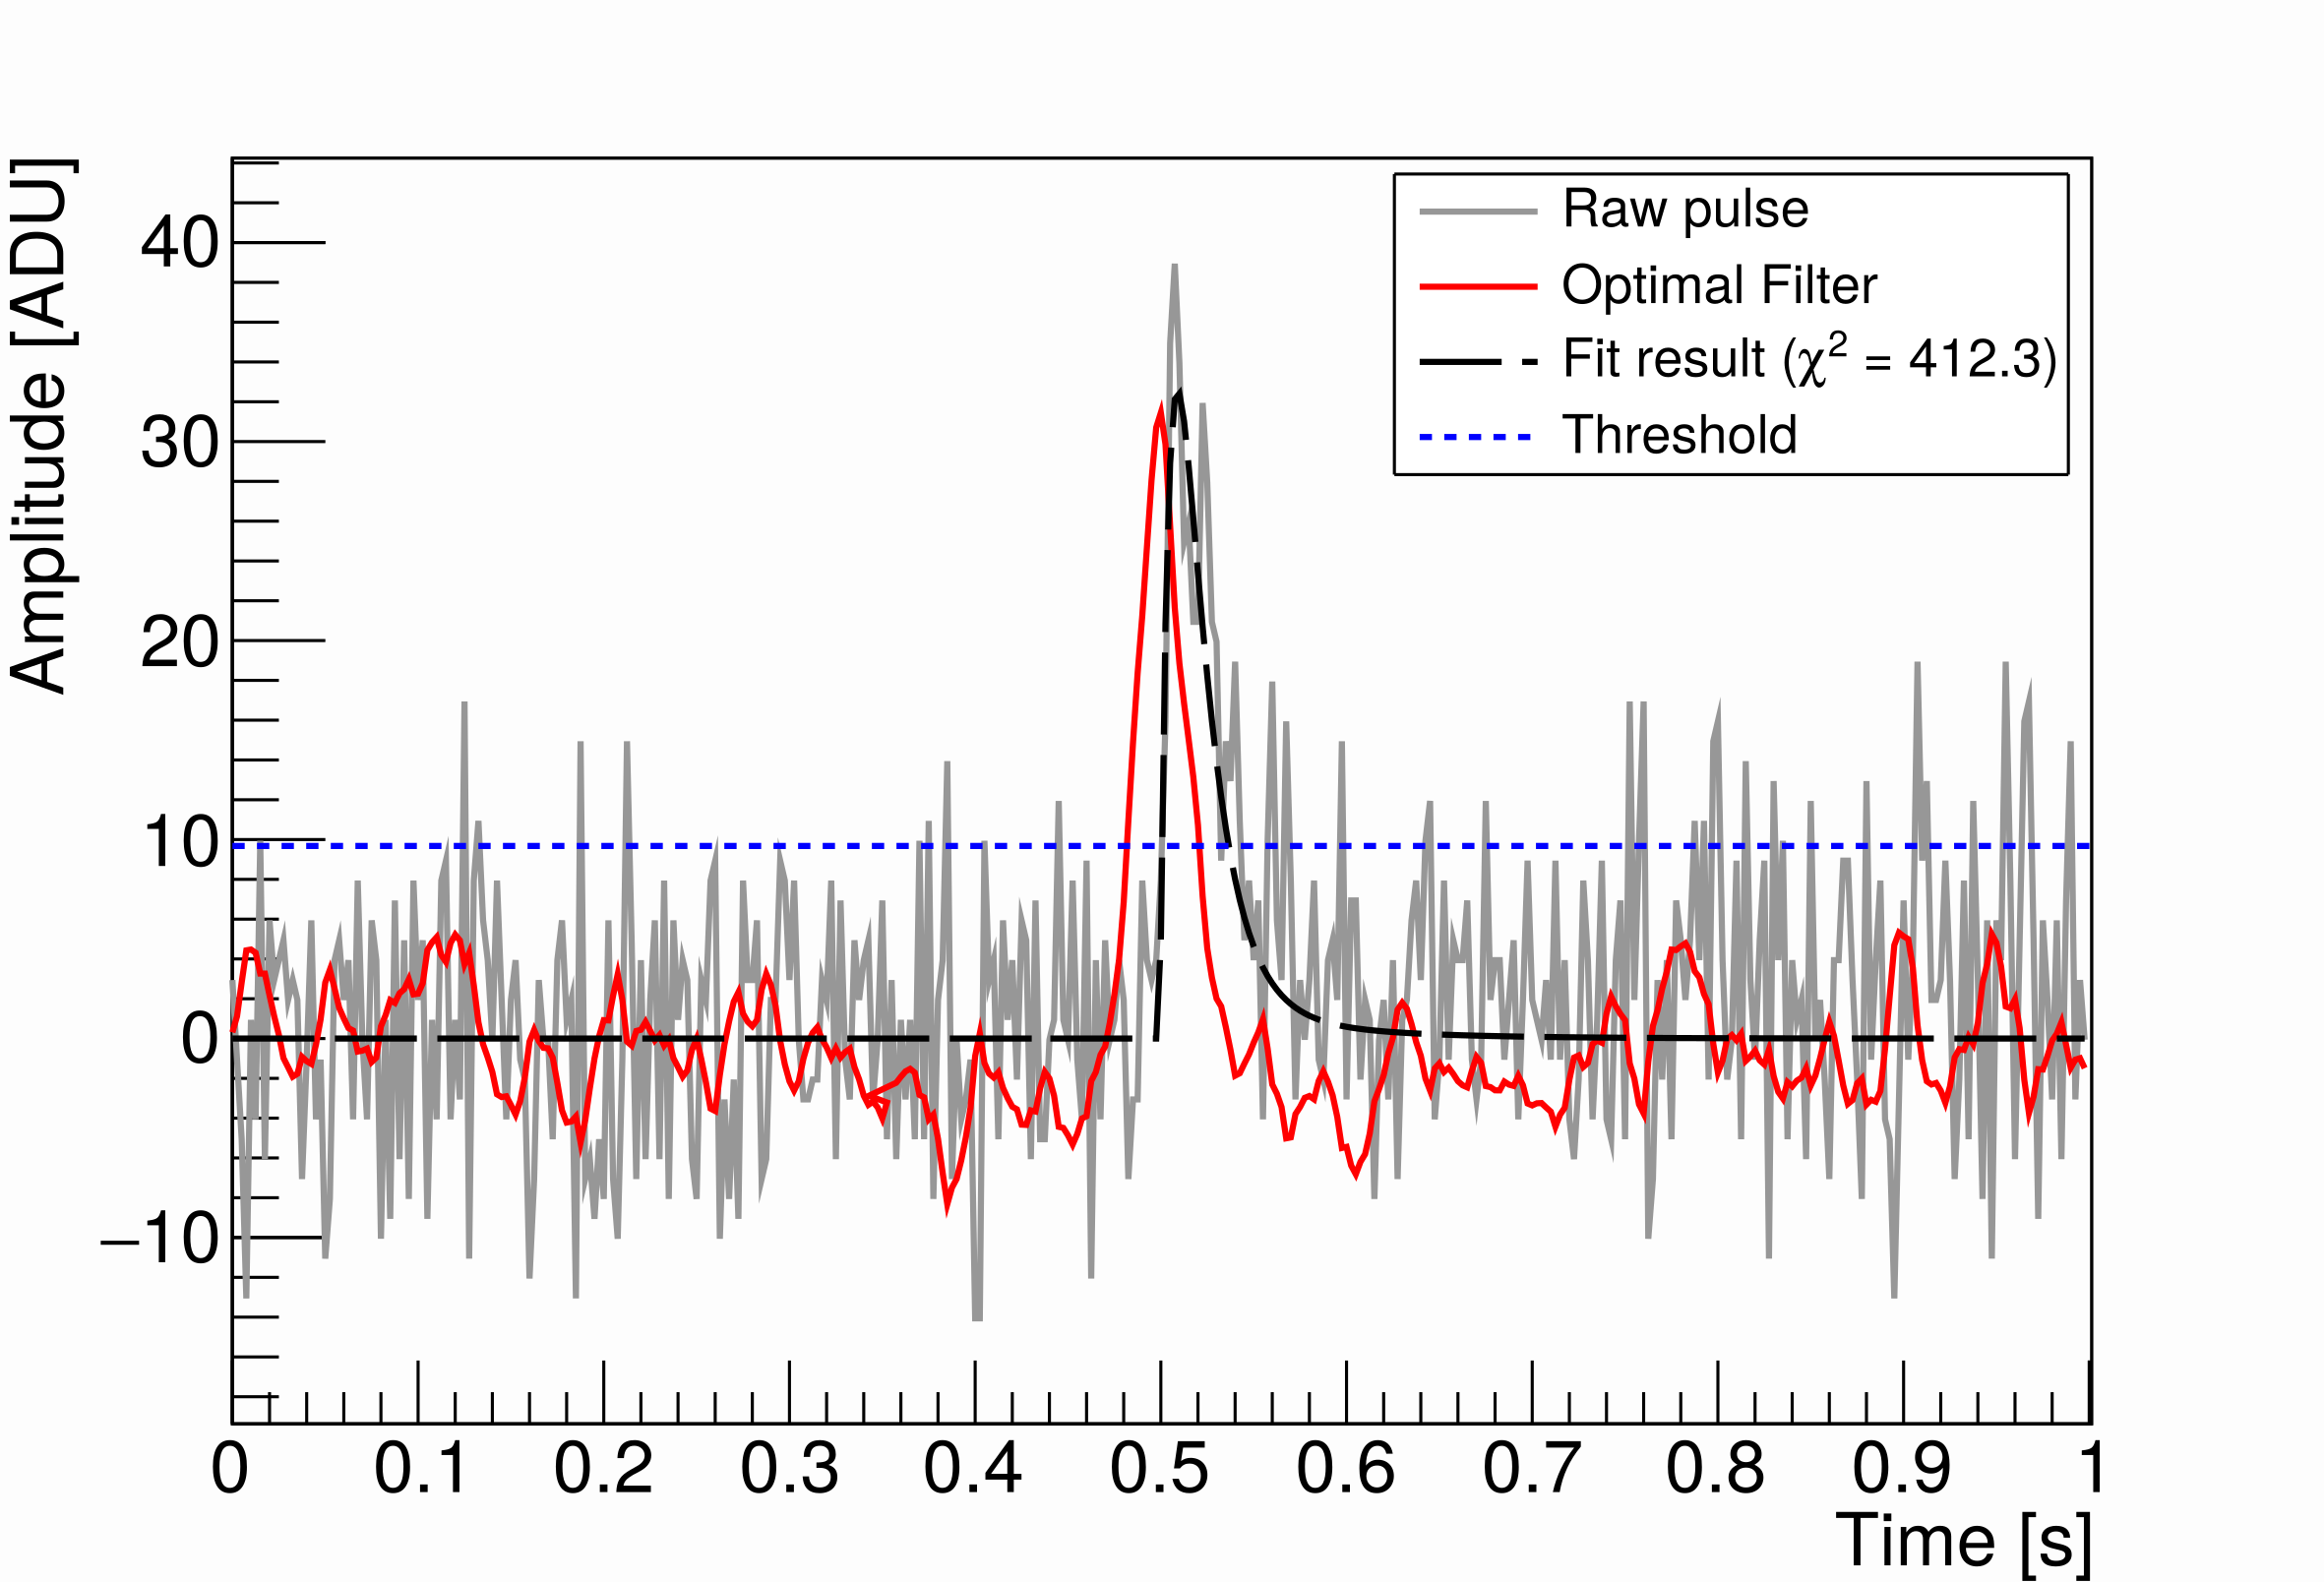
\includegraphics[width=\linewidth,]{Figures/Neutron/pulse_of.png}
\caption{TO DO: Raw and Optimal filtered of a 1s pulse window with legend of important amplitude and times, used for the quality cuts.}
\label{fig:raw-of-signal}
\end{figure}

These time windows are processed to extract several quantities:
\begin{itemize}
	\item Timestamp,
	\item Amplitude (filtered decorrelated),
	\item Chi2 value (filtered decorrelated),
	\item Offset (raw),
	\item Ionization Slope (raw),
\end{itemize}
The figure \ref{fig:analysis-monitoring-demo} shows this characterization quantities for each triggering event as a function of their timestamp (for the considered stream, here tg17l007). Each scatter plots is understood when applying the quality cut:
\begin{itemize}
	\item Heat Energy vs Timestamp: Reconstruction of the energy deposited in the heat channel for each event. This graph can be linked to the heat energy spectrum presented later. One can note pronounced population of fixed energy corresponding to the abundance of 10.37keV events due to the activation of the Germanium crystal and the noise blob poulation at $\mathcal{O}(50)$eV.
	\item Ionization Energy vs Timestamp: is quite the same as heat energy, except that with the overlap of the different channels this graph is now an useless mess
	\item Offset Heat vs Timestamp: this curve is proportional to the resistance value of the NTD sensor and allows us to follow the baseline temperature. With this decreasing profile, we deduce that the detector has been cooling during this stream. Note that although RED80 is still slowly thermalizing, the sensitivity is stable (precision?)
	\item Offset Ionization vs Timestamp: this curve is essentially used to discard all the events with an offset outside of the $[-14000, 14000]$ ADU (see \ref{par:quality-cuts}).
	\item Slope Ionization vs Timestamp: this curve is proportional to the baseline current measured by each electrodes. This baseline current is explained by the presence of leakage current between the electrodes (dedicated section?) and the collection of trapped charges (especially after a maintenance).
	\item Chi2 vs Timestamp: This describes the goodness of the fit of the template to the pulse. A stable low value indicate a fixed shape for the pulses, which is required for the chi2 cut applied later (see \ref{par:quality-cuts})
\end{itemize}

\begin{figure}
\centering
%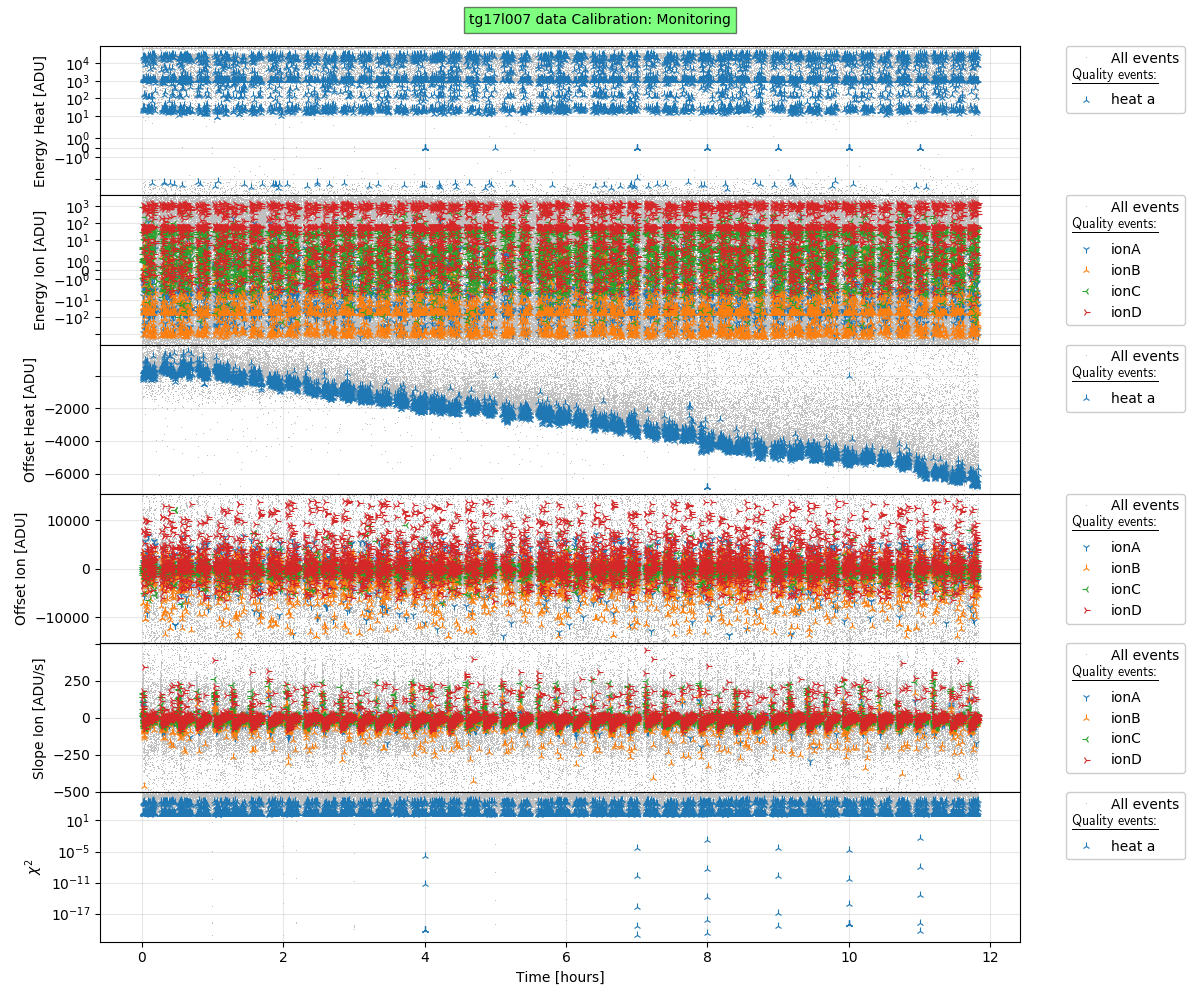
\includegraphics[width=\linewidth,]{Figures/Neutron/analysis_monitoring_demo.png}
\caption{TODO: Relevant quantities as function of the timestamp (Heat offset, slope ion, others?). Zoom for better explanation. Characterization quantities of triggering events as a function of their timestamp. (TO BE CHANGE !)}
\label{fig:analysis-monitoring-demo}
\end{figure}

In the end, for each configuration of data measurements(Background and Calibration), triggering events were selected in each streams and described by several quantities.
Among those triggering events are events of interest well reconstructed and induced by electronic recoil from the radioactive gamma background, the KLM activation lines from the germanium and the cosmic muons and neutron recoil from the AmBe neutron source and the radioactive neutron background. However, many triggering events can not be reconstructed or were induced by parasitic source, and can not yield information for the measurement of the neutron background at IP2I. To extract the events of interest from all the data, analysis cuts are applied.

Between each maintenance, the detector stays floating. The common noise can be subtracted when considering the charge conservation for all the electrodes:
\begin{equation}
\label{eq:charge-conservation}
A + B + C + D = 0
\end{equation}
With a linear combination of the raw ionization channels (A,B,C,D), we obtain new quantities (A’, B’, C’, D’) corrected from this common noise:
\begin{equation}
\label{eq:common-noise-subtraction}
A’ = \frac{3}{4} A - \frac{1}{4} \left( B + C + D \right)
\end{equation} 
The decrease of the noise level can be appreciated in the figure \ref{fig:ionization-noise} showing the noise spectrum affecting the different ionization channels before and after linear combination.


\section{Live Time Cut}


{\color{red} Need to link this to the window length of 1s. Because a shorter window length would increase the livetime at the cost of the resolution i think.}

The livetime corresponds to the period of time where the detector is considered available for data taking.
It is important to consider the appropriate livetime for a stream as all the results presented in the analysis will eventually be weighted by the exposure of the detector and so this very livetime. While we would like the livetime to corresponds to the running time of the detector, it is often not the case. There can be some periods where the temperature regulation of the cryostat can be defective (temperature spikes, power cuts) which degrade the heat sensitivity of the detector, and other periods where various malfunctions can prevent the saving of data all together. The stability of the detector operation is monitored for each streams with a graph of the energy amplitude of the events in function of their timestamp.

% Such a graph is plotted in the figure \ref{fig:analysis-monitoring-demo} for the stream "tg27l000".

%\begin{figure}
%\centering
%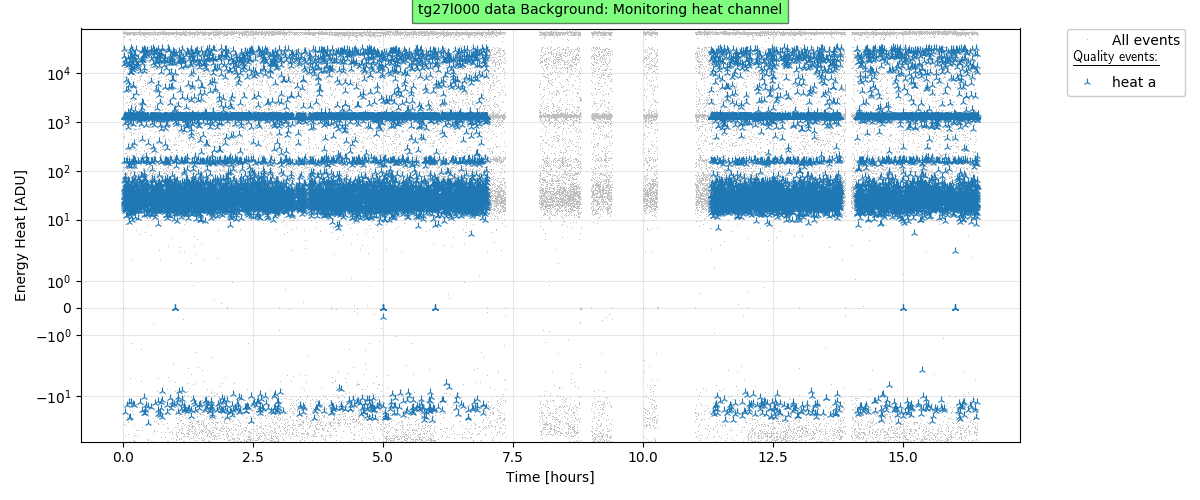
\includegraphics[width=\linewidth,]{Figures/Neutron/analysis_glitch_cut_demo.png}
%\caption{Reconstructed amplitude on the heat channel in function of the timestamp for every events of the stream "tg27l000". All events are plotted in grey while events passing the "Livetime" are in blue.}
%\label{fig:analysis-monitoring-demo}
%\end{figure}

It appears that RED80 was operated at a constant temperature for the duration of this stream (this is also observed for all the other streams). Indeed, the events corresponding to the calibration peaks are reconstructed with a fixed amplitude (approximately $2 \times 10^2$ ADU for the 1.3keV and $2 \times 10^3$ ADU for the 10.37keV), and thus we check that the sensitivity of the heat channel is constant for the whole stream.

However, some strange periods of time are visible where no events were saved. In the presented figure, it is most notable in the intervals $[7, 11.3]$ and $[13.8, 14.1]$ hours. These portions of the streams were corrupted or rendered useless for reasons not clearly understood relative to the acquisition electronics.

The livetime is visually deduced from this monitoring plot for each stream and presented in the table \ref{tab:stream-glitch-time-cut}.

\begin{table}[]
\centering
\resizebox{\linewidth}{!}{
	\begin{tabular}{l|cc|r|r|r|l|r}
\multicolumn{1}{c|}{\multirow{2}{*}{Stream}} &
  \multicolumn{2}{c|}{Time Interval {[}hours{]}} &
  \multicolumn{2}{c|}{Time length {[}hours{]}} &
  \multicolumn{1}{c|}{\multirow{2}{*}{\begin{tabular}[c]{@{}c@{}}Livetime\\  Percentage\end{tabular}}} &
  \multicolumn{1}{c|}{\multirow{2}{*}{Configuration}} &
  \multicolumn{1}{c}{\multirow{2}{*}{Livetime}} \\ \cline{2-5}
\multicolumn{1}{c|}{} &
  \multicolumn{1}{c|}{Raw} &
  Fine &
  \multicolumn{1}{c|}{Raw} &
  \multicolumn{1}{c|}{Fine} &
  \multicolumn{1}{c|}{} &
  \multicolumn{1}{c|}{} &
  \multicolumn{1}{c}{} \\ \hline
tg17l007 &
  \multicolumn{1}{c|}{{[}0, 11.83{]}} &
  {[}0, 11.83{]} &
  11.83 &
  11.83 &
  100\% &
  \multirow{4}{*}{Calibration} &
  \multirow{4}{*}{75.6} \\
tg19l010 &
  \multicolumn{1}{c|}{{[}0, 20.86{]}} &
  {[}0, 8.3{]} $\cup$  {[}8.7, 20.86{]} &
  20.86 &
  20.47 &
  98.1\% &
   &
   \\
tg20l00 &
  \multicolumn{1}{c|}{{[}0, 26.37{]}} &
  {[}0, 26.37{]} &
  26.37 &
  26.37 &
  100\% &
   &
   \\
tg21l000 &
  \multicolumn{1}{c|}{{[}0, 16.93{]}} &
  {[}0, 16.93{]} &
  16.93 &
  16.93 &
  100\% &
   &
   \\ \hline
tg18l005 &
  \multicolumn{1}{c|}{{[}0, 14.95{]}} &
  {[}0, 7.4{]} $\cup$ {[}7.6, 14.95{]} &
  14.95 &
  14.75 &
  98.7\% &
  \multirow{3}{*}{Background} &
  \multirow{3}{*}{35.93} \\
tg27l000 &
  \multicolumn{1}{c|}{{[}0, 16.43{]}} &
  {[}0, 7{]} $\cup$ {[}11.3, 13.8{]} $\cup$ {[}14.1, 16.43{]} &
  16.43 &
  11.83 &
  72.0\% &
   &
   \\
tg28l000 &
  \multicolumn{1}{c|}{{[}0, 21.50{]}} &
  {[}0, 7.4{]} $\cup$ {[}8.05, 10{]} &
  21.50 &
  9.35 &
  43.5\% &
   &
  
\end{tabular}
}
\caption{Calculation of the livetime of every stream. Fine time intervals were estimated visually from monitoring plots (as in figure \ref{fig:analysis-monitoring-demo}) with precautionary buffers. The "Livetime cut" keeps all the events with timestamps in the selected fine intervals. The total lifetime of both configuration is used in the calculation of the exposure of the RED80.}
\label{tab:stream-glitch-time-cut}
\end{table}

%\begin{table}[]
%\centering
%\resizebox{\textwidth}{!}{%
%\begin{tabular}{l|l|l|l|l}
%Configuration & Stream & Selected Intervals / h & Live time percentage & Total Live time / h \\ \hline
%\multirow{3}{*}{Background}  & tg18l005 & lol & 98.7 & \multirow{3}{*}{75.6}  \\
%                             & tg27l000 & lol & 72.0 &                        \\
%                             & tg28l000 & lol & 43.5 &                        \\ \hline
%\multirow{4}{*}{Calibration} & tg17l007 & lol & 100  & \multirow{4}{*}{35.93} \\
%                             & tg19l010 & lol & 98.1 &                        \\
%                             & tg20l000 & lol & 100  &                        \\
%                             & tg21l000 & lol & 100  &                       
%\end{tabular}%
%}
%\caption{}
%\label{tab:my-table}
%\end{table}

The raw streams have various "fine" time intervals where the data can be taken properly. These fine intervals define the so-called "Livetime cut" which discarded any events not in the fine intervals. In the figure \ref{fig:analysis-monitoring-demo}, all the events are plotted in gray while only the events passing the Livetime cut are plotted in blue. The intervals were chosen with some precautionary buffer in to apply a conservative cut that would reject any abnormal event. In the end, the livetime is obtained for each streams and added for both configuration, giving a livetime of $75.6$ hours for the Calibration and $35.93$ hours for the Background.



\section{Quality Cuts}
\label{par:quality-cuts}

The objective of the "Quality cut" is to keep the events induced by recoils in the germanium absorber of RED80 and with a good energy reconstruction. These events  passing the Quality cut are labeled as "quality events" and satisfy several criteria:
\begin{itemize}
	\item passing the Livetime Cut,
	\item not happening during a maintenance period of the ionization channel,
	\item offset of the ionization channel in the $[-14000, +14000] ADU$ interval,
	\item the $\chi^2$ value, expressing the goodness of the fit of the event with the signal template.
\end{itemize}

{\color{red} Maintenance cut paragraph, will surely be moved in the section describing the electronics.}
\label{par:reset-maintenance}
The electrodes of the ionization channel are collecting the electron-hole pairs induced by the recoils in the germanium crystal. As a results, their electric potential is decreasing (recall $Q=CU$) as well as the electric field guiding the e-h pairs in the crystal. In order to keep a steady electric field, it is necessary to periodically recharge the electrodes, offsetting the effect of the e-h pairs collection. This process is called "Reset" and is usually set to happen every few seconds in detectors.
An adverse effect of these resets is that they usually induce a signal on the heat and ionization channels. While these signals are easily discarded using their known frequency, they can happen close to a valid signal resulting in a pile-up, the discarding of the event from the analysis, and so a decrease in the livetime of a data stream.

Another phenomenon degrading the electric field is the trapping of the charges in the crystal. Even if the electrodes are properly "resetted", the accumulating trapped charges produces a counter-field effectively reducing the electric field seen by the e-h pairs in the crystal. The method used to even the charges in the crystal is called "Maintenance". The electrodes are successively polarized at plus and minus their nominal electric potential with a frequency of $\mathcal{O}(1\textsf{Hz})$ for about a minute. The trapped charges are shaken up in the crystal and eventually recombine or are collected at the electrodes. The counter-field vanishes and the detector is ready to operate with its standard electric field (graph necessary to illustrate ?). A downside is that the detector is not available for data taking during a maintenance, representing about a minute of deadtime for several tenths of minutes of running time. 

As this work uses data taken with detectors operated in an above-ground laboratory, the event rate is higher compared to an underground facility due to the abundance of cosmic rays and the natural radioactivity.
With this higher event rate  comes a higher charge collected per unit of time. This induces a quicker decrease of the electric potential of the electrodes, which needs for more frequent resets, and a quicker appearing of the counter-field due to the charge trapping, which calls for more frequent maintenances.

Thus, the frequency of the reset and the maintenance is adapted to the event rate seen by the detectors. The reset and maintenance should be frequent enough to keep up with the electric field decrease, yet spaced out to keep a reasonable livetime. Moreover, the event rate do fluctuate between each run as it depends on the mass of the absorbers (here 32g, 38g or 200g) and the possible use of calibration sources increasing the event rate (see the section \ref{par:calibration-sources}).
In average in this work, the resets are set to a frequency of $2$Hz (?) and maintenance set to take place every 40 minutes.
{\color{red} End of Maintenance paragraph}

Quality events should not happen during a maintenance period nor a reset (introduced in section \ref{par:reset-maintenance} as they are considered electronics artifacts. The "Maintenance cut" is defined as:
$$ bli blou bloup$$
which discards any event happening during a maintenance period.
The "Reset cut" is expressed as:
$$ hello there general$$
which discards event occurring within $5$ms (?) of a reset. 
{\color{red} INSERT MATHEMATICAL DEFINITION of the maintenance cut and the reset cut. And implement it correctly in the analysis! }

{\color{red} paragraph about the ion sensitivity degradation past 14000ADU. Dont know if this is gonna stay in this chapter or move it when describing the electronics. Feel like it should belong here, as I can illustrate that with a figure}

We noticed a malfunction for the ionization channel: apparently, the sensitivity of the ionization channels depends on their offset value. This behavior is consider as faulty as we expect the electrodes to have a constant sensitivity. This phenomenon is illustrated in the figure \ref{fig:offset-problem} which plots the ionization amplitudes of events as a function of their offset values for the data stream "???".

\begin{figure}
\centering
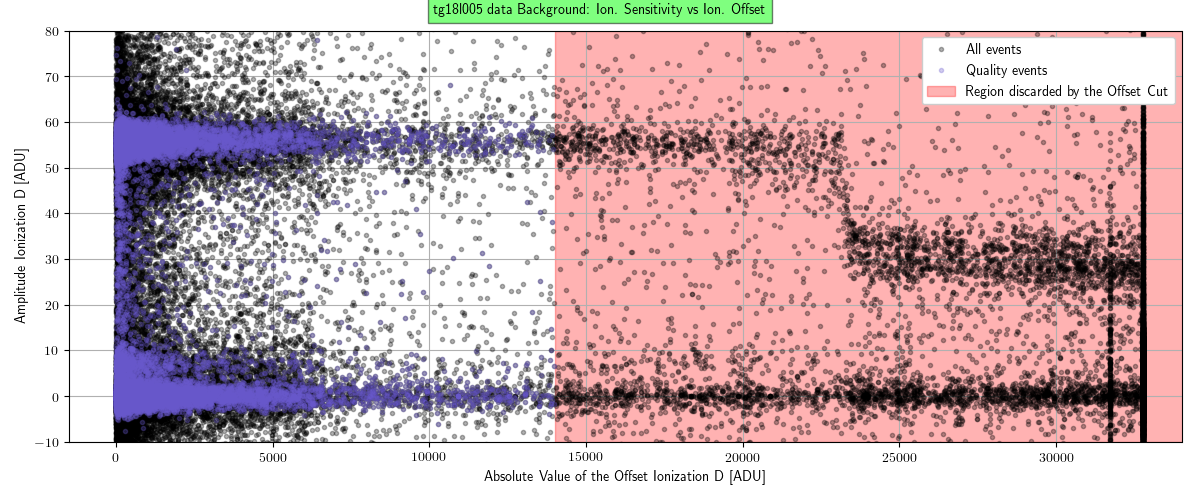
\includegraphics[width=\linewidth, height=6cm]{Figures/Neutron/offset_cut.png}
\caption{Graph of the reconstructed amplitude of the triggering events on the ionization channel D in function of their offset value. The dense population of 10keV calibration events with a reconstructed ionization energy of about 60ADU let us monitor the sensitivity of the electrodes. We note that past 23000 ADU of offset, the electrodes becomes half as sensitive as before with the 10keV calibration population reconstructed at 30ADU. The red overlay span illustrates the region discarded by the offset cut.The data presented corresponds to the stream "tg18l005". }
\label{fig:offset-problem}
\end{figure}

INTERPRETATION when plot is ready.
We decide to keep the events with the standard ionization sensitivity with low absolute offset value. Other events are discarded by the "Offset cut" which is expressed as:
$$ mathemics here $$


Concerning the $\chi^2$ value, the threshold depends on the energy. Indeed, because of non-linearity in the bolometer heat response, the shape of the signal do depends on the recoil energy as the first order perturbation theory becomes less and less valid.
Good events at low energy should have a $\chi^2$ value of about:

\begin{equation}
\mathbb{E}\left( \chi^2 \right) 
= N_{\textsf{samples in window}}
 = T_{\textsf{window}} \times f_{\textsf{sampling}}
 = 0.5 \times 400 = 200
\end{equation}

However, with a signal template based on events from the 10.37keV activation line of the germanium, the $\chi^2$ value of good events is increasing from $\mathcal{O}(10keV)$.
Therefore, a cut parametrization function depending on the event amplitude is chosen:

\begin{equation}
Threshold(Amplitude) 
= \gamma \times \mathbb{E}\left( \chi^2 \right)  \times \left[ 1+ \left( \frac{Amplitude}{\alpha} \right)^\beta \right]
\end{equation}

with $\alpha$, $\beta$ and $\gamma$ estimated visually for each streams and presented in table \ref{tab:chi2-cut}.

\begin{table}[]
\centering
\begin{tabular}{l|l|l|l|l}
Channel type                & $\alpha$                         & $\beta$              & Streams              & $\gamma$           \\ \hline \hline
\multirow{7}{*}{Heat}       & \multirow{7}{*}{$2 \times 10^3$} & \multirow{7}{*}{2}   & tg17l007             & 1                  \\
 &  &  & tg18l005 & 1    \\
 &  &  & tg19l010 & 1    \\
 &  &  & tg20l000 & 1    \\
 &  &  & tg21l000 & 1    \\
 &  &  & tg27l000 & 1.75 \\
 &  &  & tg28l000 & 1.75 \\ \hline
\multirow{7}{*}{Ionization} & \multirow{7}{*}{$3 \times 10^2$} & \multirow{7}{*}{2.2} & \multirow{7}{*}{All} & \multirow{7}{*}{1} \\
 &  &  &          &      \\
 &  &  &          &      \\
 &  &  &          &      \\
 &  &  &          &      \\
 &  &  &          &      \\
 &  &  &          &     
\end{tabular}
\caption{Coefficient of the $chi^2$ cut for each streams. These coefficients were determined visually in order to defined the band of events of lowest $chi^2$ value on the whole energy range.}
\label{tab:chi2-cut}
\end{table}


In the end, the $\chi^2$ cut is applied on each channels (as seen in figure \ref{fig:chi2-cut}) independently. Only the events passing the cut for all the channels is kept and eligible as a quality event.

\begin{figure}
\centering
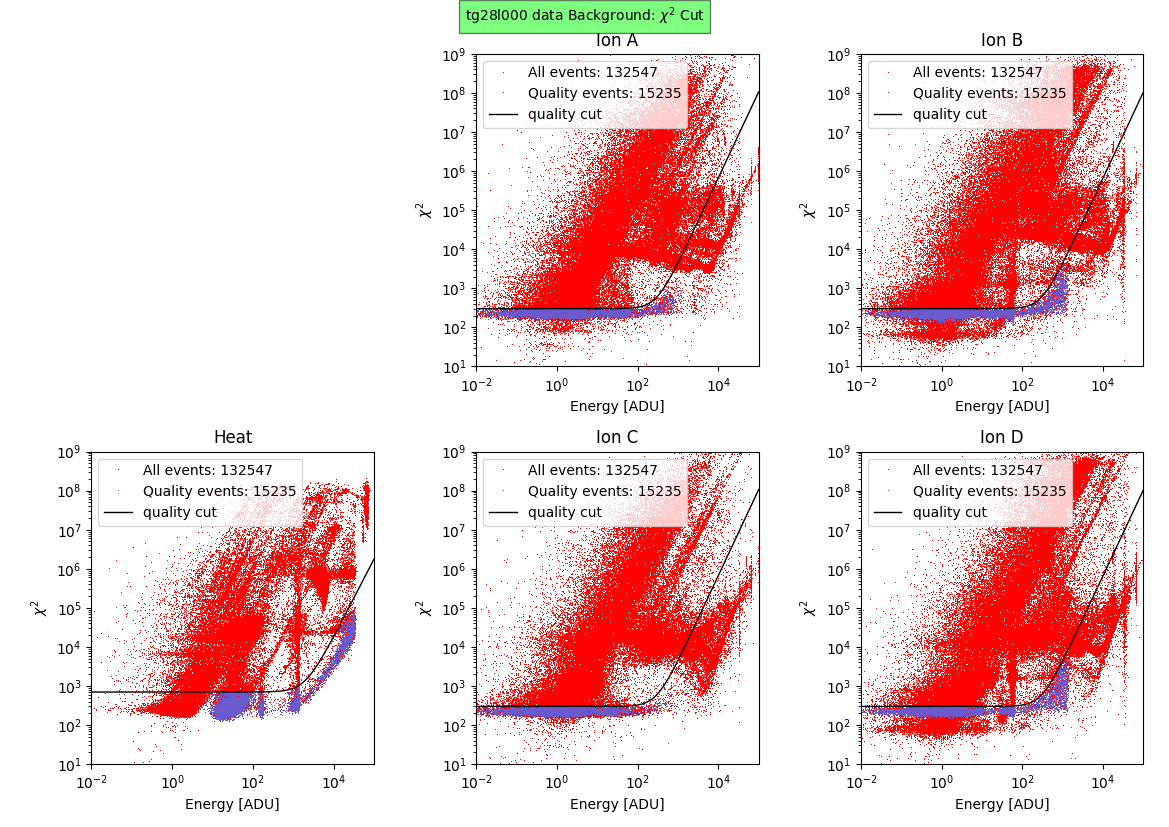
\includegraphics[width=\linewidth,]{Figures/Neutron/chi2_cut.png}
\caption{$\chi^2$ value for each event in function of its reconstructed amplitude for the five measuring channels. The cut threshold is represented by the black line. All events are in red, passing events are in blue.}
\label{fig:chi2-cut}
\end{figure}

With all these criteria being applied to the events passing the Livetime Cut, we have selected the events passing the Quality Cut, qualified as "quality events".

TO DO: merge with chi2 cuts from the previous Chapter Electrodes Experimental.
(threshold function = cut parametrization)

\section{Cross-talk Correction}
\label{par:crosstalk}

See cross-talk explanation in the Chapter \ref{ChapterElectrodesExperimental}.


\section{Calibration}
\label{par:calibration}

The five measurements channels are saving the voltage of their associated sensors in ADU unit specific to each considered channel. In order to proceed with physical interpretation, it is now necessary to convert the channels into a common unit.
For this purpose, we use the activation of the KLM lines of the Germanium crystal, which emits a gamma of energy 100eV, 1.3keV and 10.37keV respectively [\cite{germanium-decay}]. This gammas of known energy produce electronic recoils depositing a known energy in the ionization channels and the heat channel, with the latter being boosted with the Luke-Neganov effect [\cite{luke-neganov-effect} and \citep{luke-neganov-interpretation}]. As the quenching of the electronic recoil is different from the one of the nuclear recoil, we use the $keV_{ee}$ which precise that the energy deposit done with an electronic recoil.

Concerning the ionization channels, we use the 10.37keV line forming a multivariate normal distributed blob in the figure \ref{fig:calibration-ion} showing the signal of an event in each ionization channel in ADU unit. We estimate the center of this distribution to be $55$ ADU for each channels. We can now deduce the calibration coefficient for the ionization channels : $\pm 55 ADU \leftrightarrow 10.37 keV_{ee}$.

\begin{figure}
\centering
\caption{TO DO Corner plot of the reconstructed ionization amplitude of the quality events, zoomed on the 10.37keV calibration peak.}
\label{fig:calibration-ion}
\end{figure}

As for the heat channel, we use the 10.37keV line forming a normal distribution visible in the ADU amplitude spectrum of the heat channel as seen in figure \ref{fig:calibration-heat}. The estimated center of this distribution is $1200$ ADU. The calibration coefficient for the heat channel is therefore: $1200 ADU \leftrightarrow 10.37 keV_{ee}$.

\begin{figure}
\centering
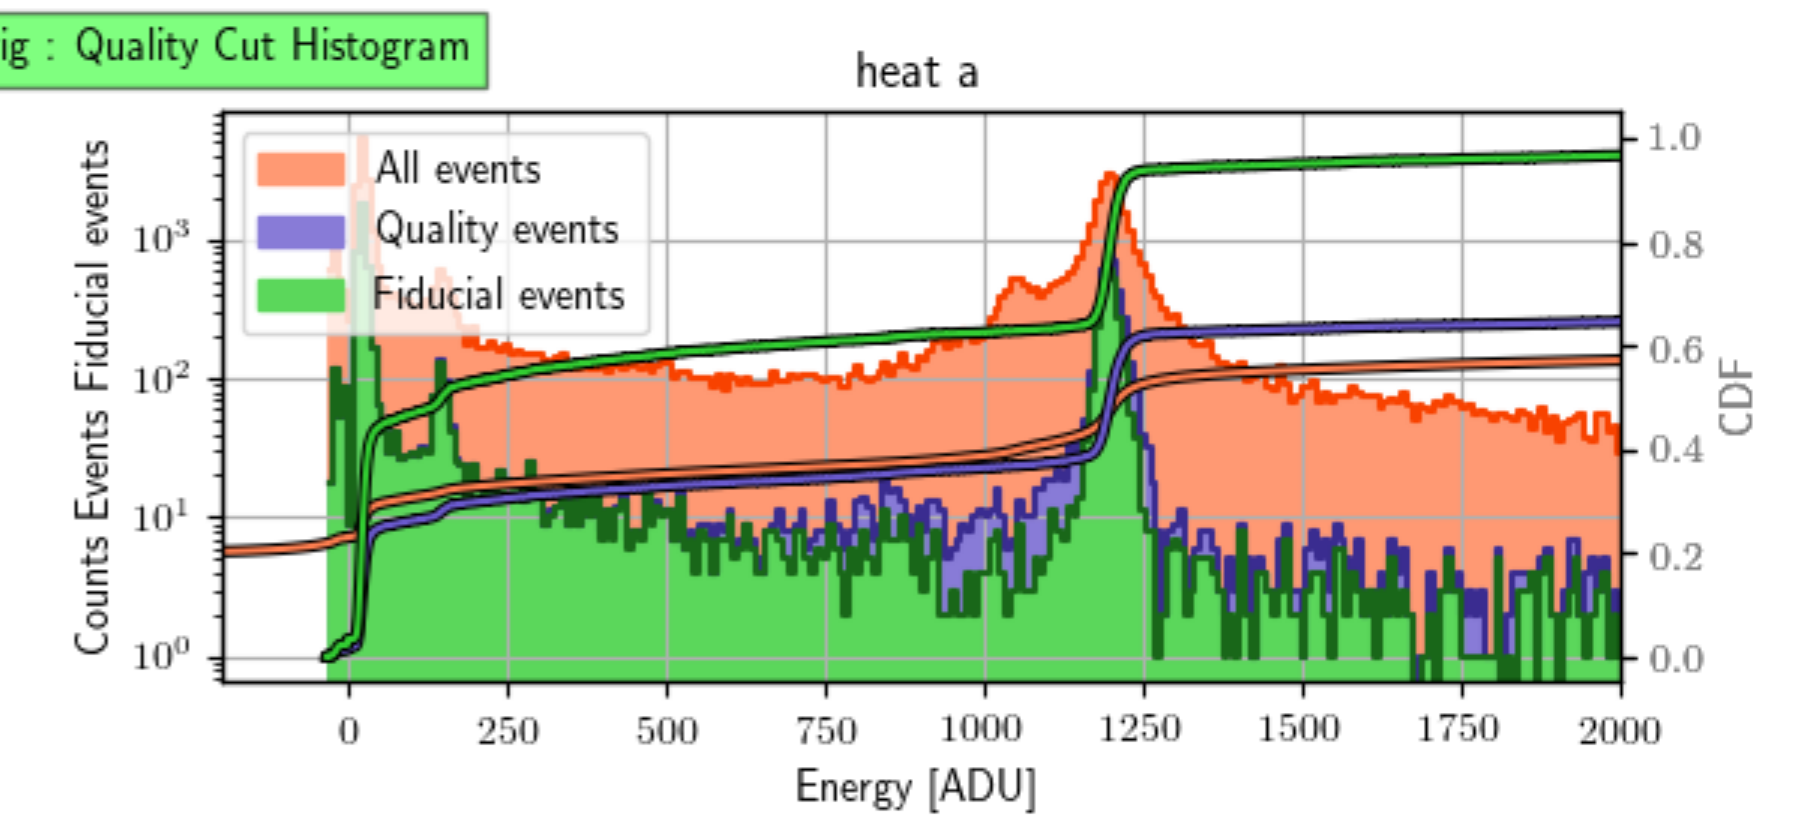
\includegraphics[width=\linewidth,]{Figures/Neutron/calibration_heat.png}
\caption{Heat Amplitude Spectrum for a stream. The calibration coefficient is estimated from the 10.37keV calibration peak position.}
\label{fig:calibration-heat}
\end{figure}

With these calibration coefficient, it is now possible to reason with the reconstructed energy for each channels as
$$
\textsf{Reconstructed energy [keV]}
=
\textsf{Calibration Coefficient [keV/ADU]}
\times
\textsf{Event Amplitude [ADU]}
$$
Now that the events of all the streams are calibrated, they are expressed in the same unit and can be compared. From now on, we concatenate the calibrated streams and consider all the events for the Background and the Calibration configurations.


\section{Charge conservation cut}
\label{par:charge-conservation-cut}

to be corrected vvv
Even with the bulk cut, some events might still have charge collection issue. Drifting charges can be trapped in the germanium and may not end up being collected. On way to discard such events is to consider the "Charge Conservation" quantity, defined as:
\begin{equation}
\mathcal{C.C.} = \frac{-A-B+C+D}{2}
\end{equation}

As a recoil produces electron-hole pairs, the charge of the drifting particles in the crystal should be zero as well as the total collected charges (considering their complete collection). This is characterized by a the normal distribution of the $\mathcal{C.C}$ around zero with an STD depending on the RMS resolution of the ionization channels. Events with an incomplete charge collection would stand out of this gaussian profile and can be discarded. As a result, we define the event passing this "Charge conservation cut" with a $\mathcal{C.C.}$ lower than two times the RMS resolution for the considered heat energy. This cut is represented in the figure \ref{fig:charge-conservation}.

\begin{figure}
\centering
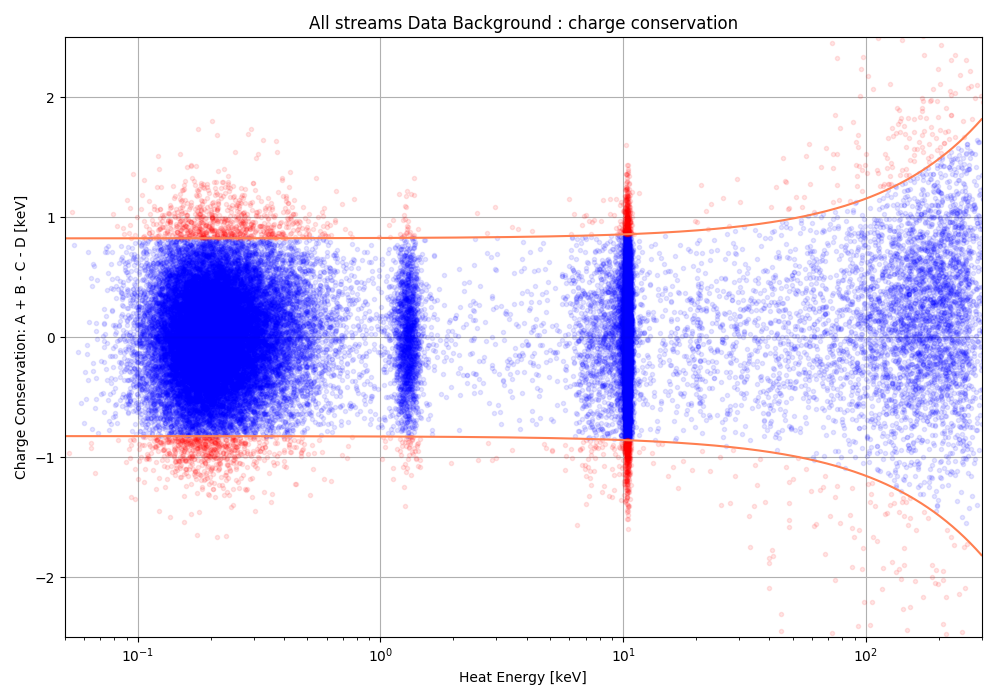
\includegraphics[width=\linewidth,]{Figures/Neutron/charge_conservation.png}
\caption{"Charge conservation" quantity as a function of the heat energy for the bulk quality events of the Background configuration. Passing events are in blue while discarded events are in red.}
\label{fig:charge-conservation}
\end{figure}

As the RMS resolution depends on the energy associated to the event, it is once more necessary to model it with a linear law:
\begin{equation}
\sigma_{\mathcal{C.C.}}\left(E_{heat}\right)
=
a + b*E_{heat}
\end{equation}
with the coefficient $a$ and $b$ coming from the estimation of the RMS resolution at 0keV (noise blob) and 10.37keV (calibration peak) (precision necessary here).


\section{Fiducial Cut}
\label{par:fiducial-cut}

Referring to the streamlines of the electric field in the crystal of RED80 (see Figure \ref{fig:streamlines-red80}), we expect some region of the crystal with a specific drifting behavior. Represented in the Figure \ref{fig:scheme-red80}, we have:
\begin{itemize}
	\item the Bulk region, where the charge will drift towards the collect electrodes B and D,
	\item the Guard region, where the charge will be collected by the surface electrodes A and C,
	\item the Corner regions, where and , we expect the charges to recombine on place of the recoil because of the very weak electric field or become trapped on the surface by drifting along the streamlines exiting the crystal.
\end{itemize}

Surface regions are always hazardous for charge collection. Indeed, EDELWEISS has a knowledge (ref necessary) of charges drifting close to the surface devoid of electrodes being easily trapped and not being collected. This behavior is degrading the ionization signal leading to a recoil with reduced quenching factor. This means that electronic recoils happening near the surface could be reconstructed with a lower quenching and be identified as nuclear recoils. The major source of such surface recoil are the $\beta$ radiation induced by the natural radioactivity interacting in the first $\mu$m of the germanium crystal (ref edelweiss necessary). Thus, we want to discard any event that may be induced by a surface recoil. When interacting on the lateral surface of the germanium crystal, this events should be collected by the guard electrodes A and C. Referring to the scheme \ref{fig:scheme-red80}, the objective of the "Fiducial cut" is to discard events from the Surface zones and Corners, and keep the events induced by recoil in the bulk region of the crystal. This Fiducial cut is applied by considering the reconstructed ionization energy of the events as represented in the figure \ref{fig:fiducial-cut}.

\begin{figure}
\centering
%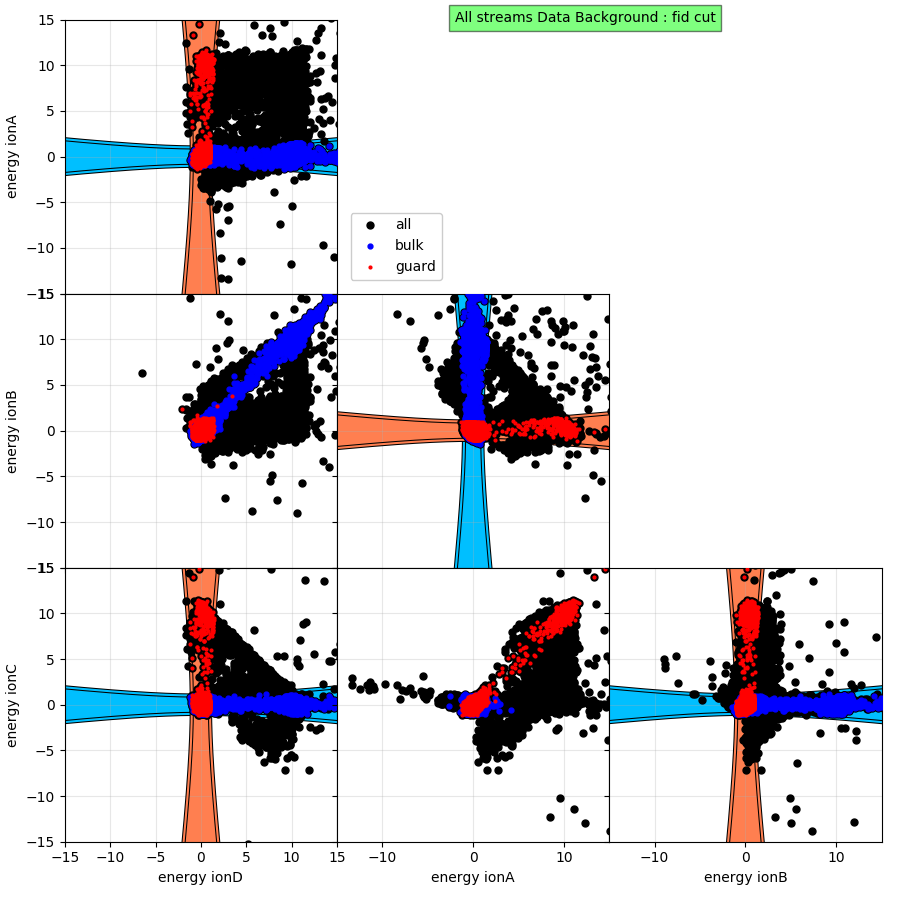
\includegraphics[width=\linewidth,]{Figures/Neutron/fid_cut.png}
\caption{TO DO: Regional cut plot. Corner plot of the reconstructed ionization energy for each electrodes for the quality events of the Background configurations. The energy thresholds for the cuts as well as the passing events are highlighted in the associated colors: blue for "bulk cut" and red for "guard cut".}
\label{fig:fiducial-cut}
\end{figure}

The Fiducial cut identifies events of the bulk region as events which did not deposited any signal on the guard electrodes A and C, with a tolerance of two $\sigma^{A,C}\left( \textsf{baseline} \right)$. For the bulk events, this conditions is expressed as:

\begin{equation}
mathmathmath for bulk events
\end{equation}

In a similar manner, we can also define the guard events with no signal on the collect electrodes B and D with a tolerance of two $\sigma^{B,D}\left( \textsf{baseline} \right)$. This condition then is written:

\begin{equation}
mathmathmath for guard events
\end{equation}

{\color{red}NOW, ITS GIBBERISH TIME !(yay, but to be modified)}
This "Bulk cut" will discard any event with a reconstructed energy on the guard electrodes A and C which is greater than two times the RMS resolution.
For this purpose, it is useful to define the reconstructed total ionization energy:
\begin{equation}
E_{ion., total} = \frac{A+B+C+D}{2}
\end{equation}

%\begin{itemize}
%	\item Ionization Energy in the Bulk region: $E_{ion., bulk} = \frac{B+D}{2}$
%	\item Ionization Energy in the Guard region: $E_{ion., guard} = \frac{A+C}{2}$
%	\item Total Ionization Energy: $E_{ion., total} = \frac{A+B+C+D}{2}$
%\end{itemize}

As the RMS resolution $\sigma_i$ of given channel $i$ depends on the total ionization energy deposited in the crystal, it is modeled by a power law:
\begin{equation}
\sigma_i\left( E_{i, total} \right)
=
\sqrt{ 
\left( \sigma_i(\SI{0}{\kilo\eV}) \right)^2 + 
\left( \alpha E_{ion., total} \right)^2
}
\quad \textsf{with} \quad
\alpha = \frac{\sqrt{\sigma_i(\SI{10.37}{\kilo\eV})^2 - \sigma_i(\SI{0}{\kilo\eV})^2}}{\SI{10.37}{\kilo\eV}}
\end{equation}
In this equation, the baseline resolution $\sigma_i(\SI{0}{\kilo\eV})$ is estimated with the standard deviation of the noise blob while the resolution $\sigma_i(\SI{10.37}{\kilo\eV})$ is estimated with the standard deviation of the events associated to the germanium calibration peak.
{\color{red}END of GIBBERISH, i think}

\subsection{Explanation of the 10.37 kev selection events}

We have discarded the events with a possible bad energy reconstruction energy and calibrated the remaining ones. The experimental signal obtained with the heat and ionization channels were reconstructed into heat energy $E_{heat}$ and total ionization energy $E_{ion.}$. The figure \ref{ecei-plot} shows the scatter plot of these two values for the events of the Calibration configuration.

\begin{figure}
\centering
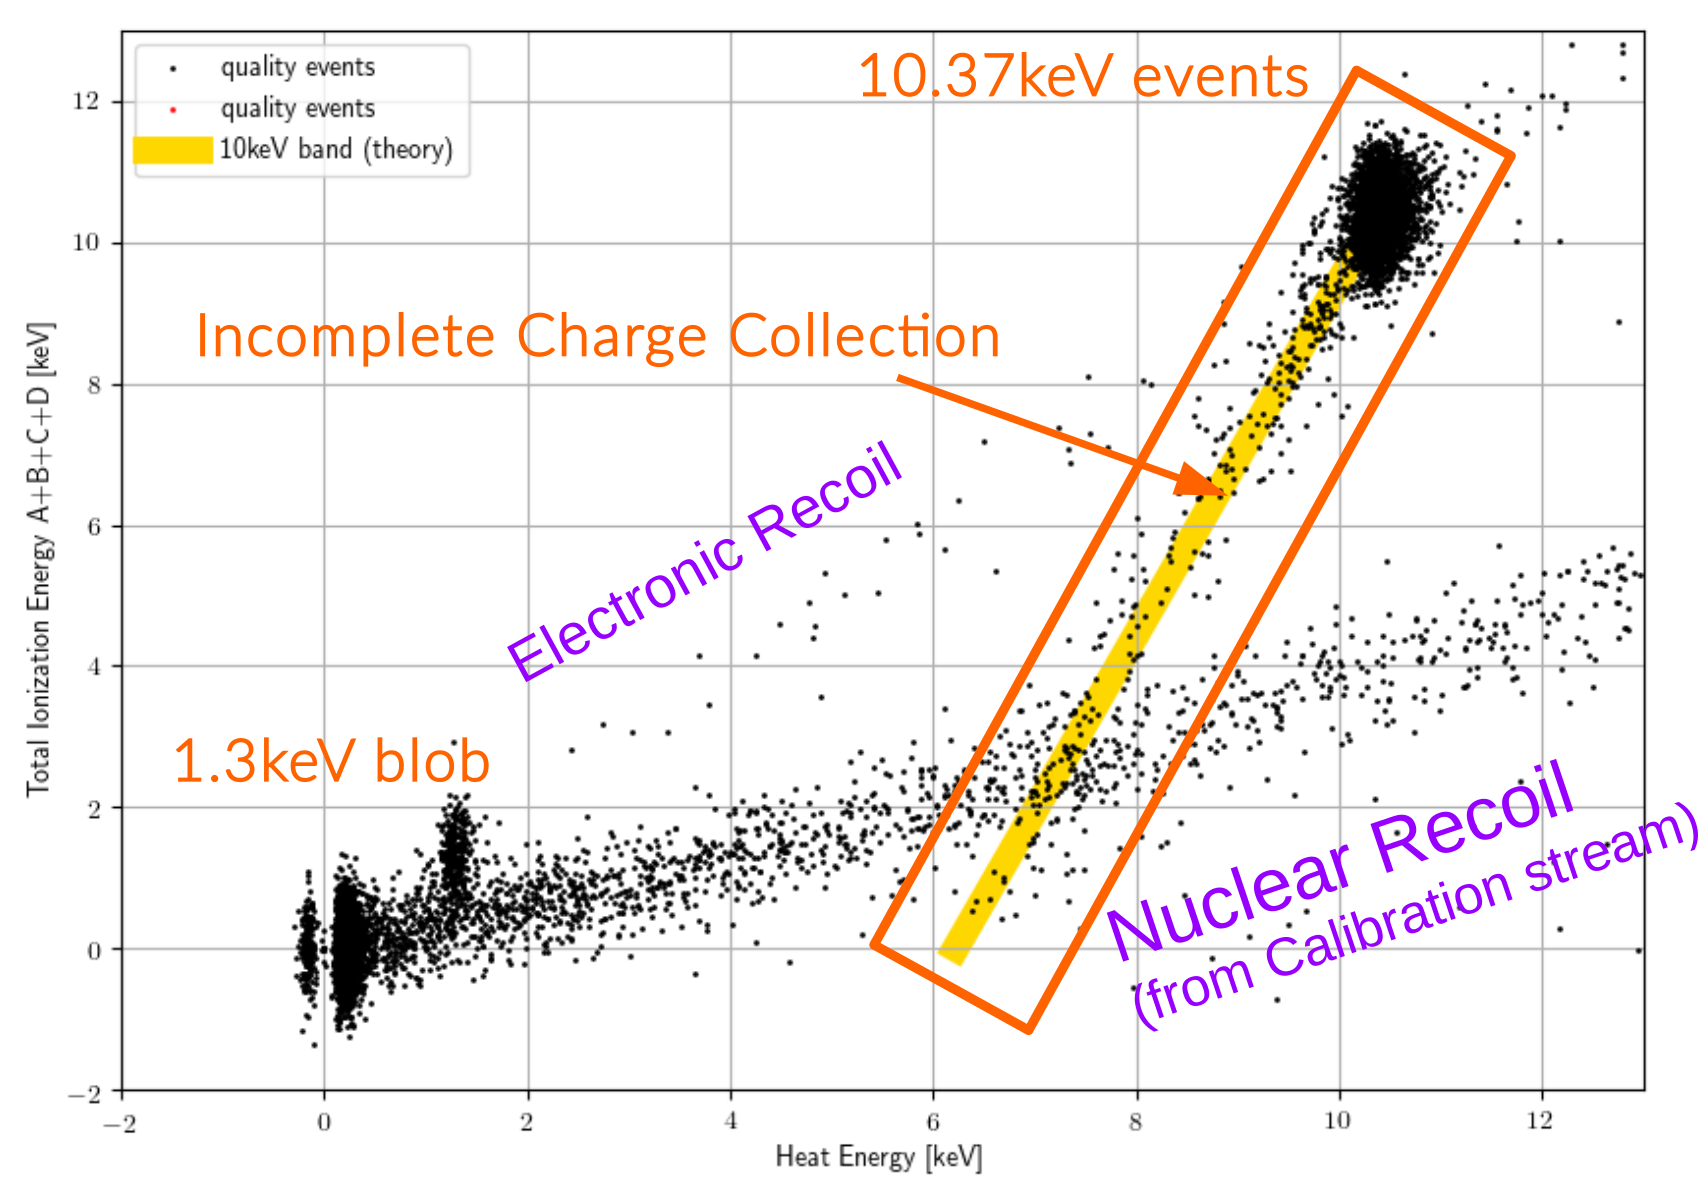
\includegraphics[width=\linewidth,]{Figures/Neutron/ecei_plot.png}
\caption{Reconstructed Ionization Energy in function of the Reconstructed Heat Energy, for the quality events of the Calibration configuration. The plot is zoomed up to 12keV for an easier view of the calibration peaks. }
\label{fig:ecei-plot}
\end{figure}

We recognize the noise blob near the origin corresponding to recoils of very low energy and triggering noise windows. Expanding from this noise blob, we note two bands. 
The electronic recoil band corresponds to events depositing the same energy in the ionization channel and the heat energy channel (both in keVee). They are characterized by a quenching factor of 1. As a matter of fact, the gamma recoil of 1.3keV and 10.37keV coming from the calibration peaks of the germanium belongs to this band. Any event below this band deposited less energy in the ionization channel than in the heat channel, and therefore possess a quenching factor inferior to one. We see that the population blob associated to the 10.37keV is smeared to lower quenching factor. This is due to events of the calibration peaks with incomplete charge collection. We note that this population is following a linear trend, which can be explained by an incomplete Luke-Neganov Boost of the heat channel according to the equation:
\begin{equation}
E_{heat} = 6 \textsf{keVee} + \epsilon \frac{2 \textsf{V}}{\epsilon_{Ge}} E_{ion.}
\end{equation}
The other major population of events below the electronic recoil band counts a lot of events in the case of the Calibration configuration. This hints that this band corresponds to the nuclear recoil induced by the AmBe neutron source.
The presence of the two bands in this plot demonstrate the discriminating ability of the associated heat and ionization channels. Note that, although the bands are well separated at high energy, they are merging at low energy due to their width which is fixed by the energy resolution of the heat and ionization channel.

Another way to represent the discrimination between the electronic and the nuclear recoil is to compute the recoil energy $E_R$ and the quenching factor $Q$ for each event:
\begin{align}
\label{eq:quenching-from-ecei}
	E_{NL} &= \frac{V}{\epsilon} ( E_{ion., ???} - E_{heat} )
	\\
	E_R = E_{heat} - E_{NL} &= E_{heat} \left( 1 + \frac{V}{\epsilon} \right) - E_{ion., ???} \frac{V}{\epsilon}
	\\
	Q &= \frac{E_{ion., ???}}{E_R}
\end{align}
with $E_{NL}$ being the heat energy boost coming from the Neganov-Luke effect \cite{luke-neganov-effect}.
The recoil energy $E_R$ is expressed in the usual $keV$ energy unit, as the Luke-Neganov Boost depending on the type of recoil was substracted from the heat energy. The Quenching factor is unitless.
The figure \ref{fig:quenching_plot} show, for each configuration, the quenching factor as a function of the recoil energy.

\begin{figure}
\centering
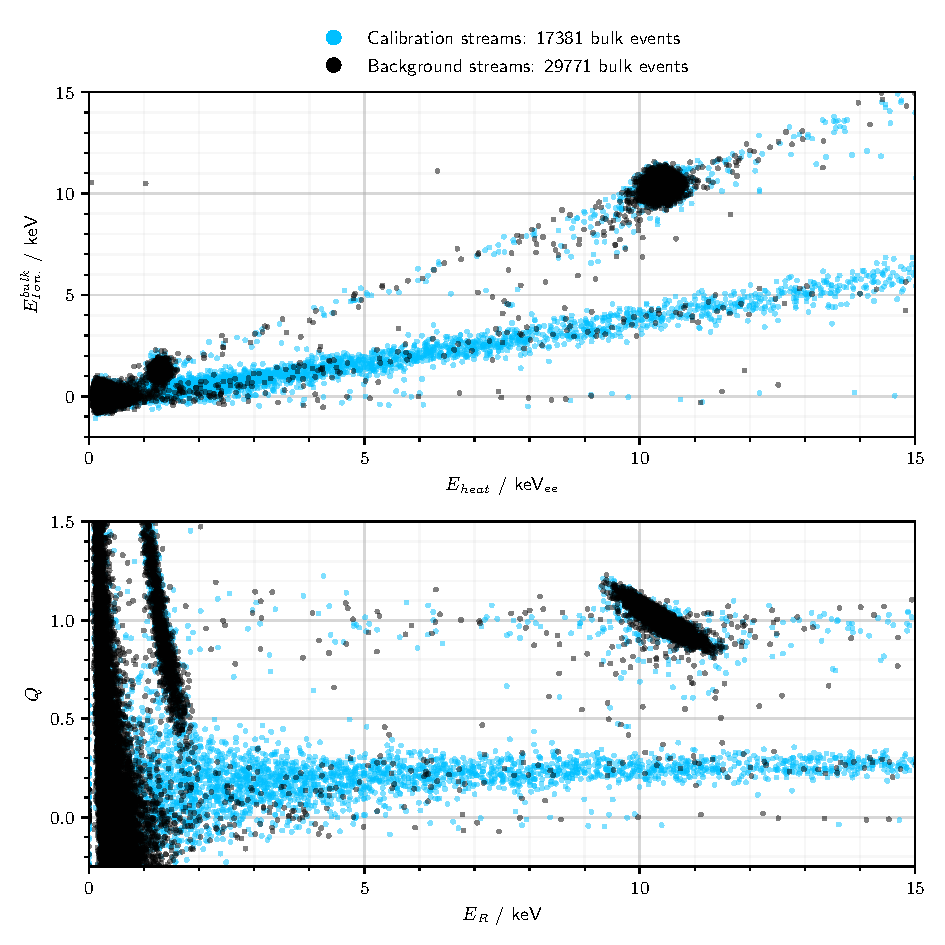
\includegraphics[width=\linewidth,]{Figures/Neutron/background_calibration_comparison.pdf}
\caption{Quenching value $Q$ for each quality events of the Background (black) and Calibration (blue) configurations in function of their recoil energy $E_R$.}
\label{fig:quenching_plot}
\end{figure}

We recognize the electronic band, centered around $Q=1$ and the nuclear recoil band with $Q<0.4$. We also note some inter-band events like the smearing of the 10.37keV events hinting at the incomplete charge collection.

%HEAT ONLY EVENT
However, there are some interesting events with a quenching factor $Q=0$ which are known as "Heat-only" events. This population is infamously known in domains in the EDELWEISS experiment [ref?] and CRESST [ref?]. This population could correspond to events with no charge collection, but this is not compatible with the lower count of inter-band events with an incomplete charge collection. An other and more realistic explanation would be the existence of energy deposit in the crystal without ionization. The source of this Heat-only event is still under investigation [ref?].

The merging phenomenon of the bands at low energy is also more visible in this graph with the change of variable. We can even visually witness that the lower part of the 1.3keV event blob is leaking into the higher part of the nuclear band.

\section{Trigger cut}
\label{par:trigger-cut}

The trigger is a pre-processing steps described in the dedicated paragraph \ref{par:trigger-step}. Its role is to detect and create the \SI{1}{\s} pulse windows, that is to say triggering event, from a data stream. The objective is this section is to decide whether a simulated event injected at a time $t_0^{input}$ has "properly" triggered or not.
On the one hand, we should discard "non-triggering" simulated event where:
\begin{itemize}
	\item the simulated pulse with a low energy could not have reach the trigger threshold, and the an earlier or later real triggering pulse was selected as closest to the injection time $t_0^{input}$
	\item a simulated pulse could have been injected near a real pulse of higher energy. As both the simulated and the real pulses are triggering and are close in time, only the real one with the highest reconstructed energy is triggering.
\end{itemize}
A maximum tolerance of $5$ms between the injection time of a simulated pulse $t_0^{input}$ and the timestamp of the closest triggering event $t_0$ was found optimal {\color{red}(cf fig + paragraph on this study)} to ensure that the triggering pulses are in fact corresponding to simulated pulses.
On the other hand, a triggering simulated event could also have been injected exactly at the same time as a real pulse of the stream, this occurrence is called a "pile-up". The resulting signal is the addition of a real and the injected pulse which will bias the energy reconstruction. A minimum time of $5$ms between the timestamp of the closest triggering event $t_0^{input}$(extracted from the stream with injected simulated pulses) and the timestamp of the closest triggering real pulse $t_0^{data}$(extracted from the original stream) was similarly chosen to discard any pile-up event.
By combining this two condition ensuring a proper triggering of the simulated event, we can define the "trigger cut" condition:
\begin{equation}
\left\{
\begin{array}{r c l}
| t_0^{input} - t_0 | &\leq& 5\textsf{ms}\\
| t_0 - t_0^{data} | &\geq& 5\textsf{ms}
\end{array}
\right.
\end{equation}
Triggering event of timestamp $t_0$ closest to a $t_0^{input}$ satisfying this condition are considered as having properly triggered.

{\color{red} nuance nece}
It is important to note that this trigger cut is specific to simulated pulses. In order to reproduce such a study with real pulses can only be done if we know the exact time of the energy deposit in the crystal. Access to this piece of information is impossible in this work using either an AmBe neutron source or the gamma calibration peak of the germanium as both this source are based on the intrinsically stochastic process of radioactive decay. However, the use of controlled source of particles could be envisioned:
\begin{itemize}
	\item facing the germanium crystal inside the cryostat, an optical fiber linked to a pulsing LED could be used as a repetitive source of electronic recoil.
	\item outside of the cryostat, a pulsed neutron source would be overkill (or would it ? idk just thinking here)
\end{itemize}

Now that we have selected the simulated pulses which properly triggered, the entire analysis chain of this very chapter \ref{ChapterNeutron} described until now is applied to these events. The triggering simulated events population is pruned of the reconstruction biased with the quality cuts and are then allocated to the ER, NR and HO bands (see Figure \ref{fig:band-cut-ecei-simu})
